\documentclass{article}
\author{Austin Hall - University of Central Arkansas}
\date{March 2020}
\title{\huge Data Analysis Project}
\usepackage{natbib}
\usepackage{graphicx}
\usepackage{amsmath}
\usepackage{epstopdf}
\usepackage{setspace}
\usepackage{indentfirst}
\usepackage{hyperref}

\doublespacing
\begin{document}
\maketitle
\begin{center}
{\LARGE Abstract}\\
\end{center}

\newpage
\section{Introduction}
\par While the relationship between sunspots and cosmicrays is well established,
the exact mechanism of this connection is lightly know compared to their
statistical connection. In this data analysis project the aim was to visualy
and quanitatively represent the cause-affect relationship of sunspots with
cosmic rays.\\
\par To acheive this, data for a specific time interval and region was 
obtained from the NOAA repositories affording a quanitative analysis.\cite{raydata} \cite{spotdata}
Sunspots are tabulated through the use of the Wolf number: $R_z=k(10g+s)$.
Where $k$ is the scaling factoring varying for location and types of intrumentation.
While $g$ representsthe number of sunspot groups and $s$ represents the number
of individual sunspots.\\
\par Using python, each data-set was filtered and
restructed for analysis. The data reflects and indirect correlation between
sunspots and cosmicray. Also, in quanitateing the correlation time between
each corresponding maximum and minimum yielded an average suggesting
a statistical gap between the two occurances.


\newpage
\section{Methods}
\par Using the files from the NOAA repository the data files were read and 
restructured with python to remove extraneous data.
Sunspots are tabulated through the use of the Wolf number: $R_z=k(10g+s)$.
Where $k$ is the scaling factoring varying for location and types of intrumentation.
While $g$ represents the number of sunspot groups and $s$ represents the number
of individual sunspots.\\

\par After proper structuring
the data was then smoothed through the use of a moving average since the 
original files contain high fluctuations within the data set.
The moving average data-set was utilized in two manners. 
Visual use came through the contruction of a subplot representing
cosmic-rays and sunspots over the course of a $50$ year period. Then was used
numerically to determine the relative maximum's and minimum's within a time
period. After determining the relative extrema the time difference between
their occurances was tabulated and averaged. 


\newpage
\section{Results}
\begin{figure}[h!]
\centering
\caption{Plot representing the data for cosmic-rays and sunspots with
blue aligning to the moving average and colored points reflecting
corresponding extrema.}
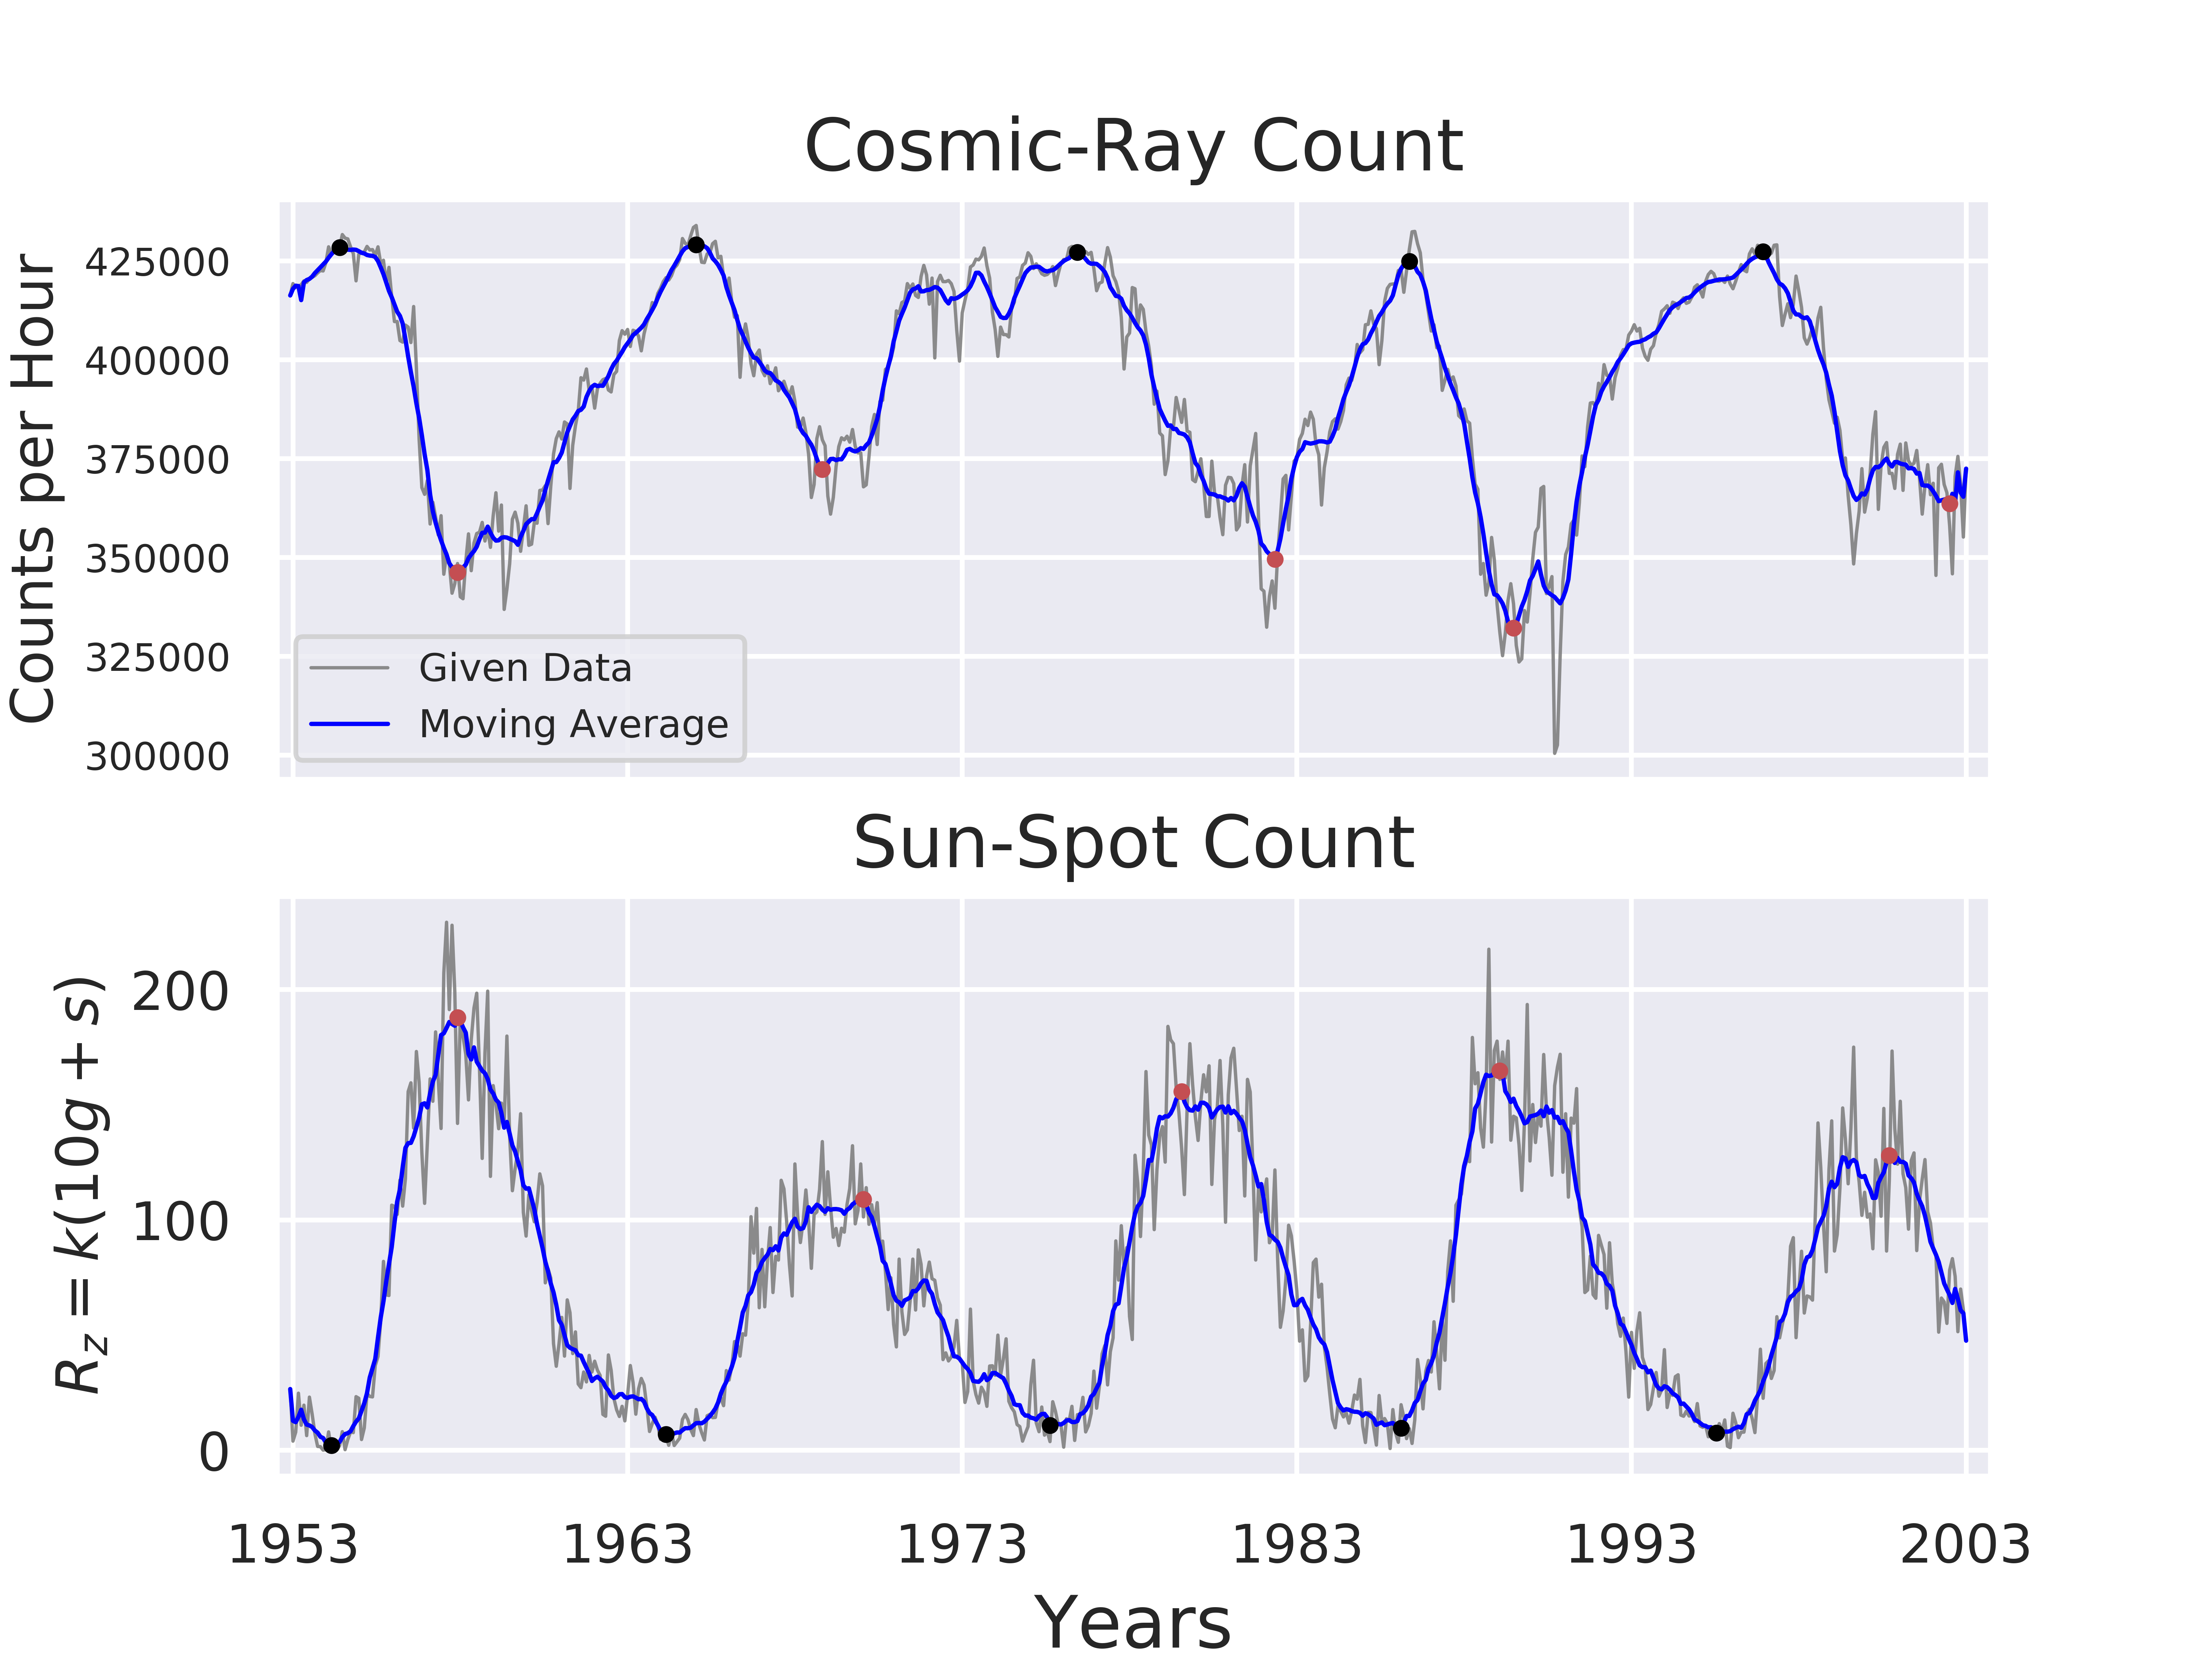
\includegraphics[scale=0.7]{plot.png}
\label{fig:sundata}
\end{figure}
\begin{table}[h!]
 \centering
 \small
 \caption{Table of corresponding extrema values and the time-gap between each.}
 \label{tbl:timegap}
 \begin{tabular}{| p{2cm} |p{2cm} |p{1cm}||p{2cm}|p{2cm}|p{1cm}|  }
  \hline
  \multicolumn{6}{|c|}{Time-Gap Data Avg=8.4 Months} \\
  \hline
  Cosmic-Ray Max's&Sun-Spot Min's&Time Gap&Cosmic-Ray Min's&Sun-Spot Max's&Time Gap\\
  \hline
  July,1954&April,1954&-3 Months&February,1958&February,1958&0 Months\\
  May,1965&June,1964&-11 Months&March,1969&June,1970&+10 Months\\
  December,1976&February,1976&-10 Months&December,1982&February,1980&-34 Months\\
  January,1987&October,1986&-3 Months&February,1990&October,1989&-4 Months\\
  October,1997&May,1996&-7 Months&June,2003&August,2001&-22 Months\\
  \hline
 \end{tabular}
\end{table}
\newpage
\section{Analysis}

In Figure \ref{fig:sundata} the gray spikes correspond to the data-set obtained
from NOAA, while the blue curves represent the moving average of each data-set.
In this figure the data curves reflect an inverse cause-affect relationship between
cosmic-rays and sunspots.\\

\par The correlation strength is further defined by the red and black
dots with each corresponding to the same color below.
Visually these dots still adhere to the correlation, however not all of
the extrema lie directly verticle to one another. Suggesting that this 
relationship is not a direct cause and affect. Table \ref{tbl:timegap} is 
utilized in exploring this connection. The average time-gap between extrema
is about $8.4$ Months. Meaning that sunspot's reach a minimum/maximum about
$255$ days before an extrema is observed in the cosmic-ray data.


\newpage
\section{Conclusion}
Through the use of open-source data and Python, a representation of the sun and it's affect on earth 
was created.
Accompanying this, extrema data suggest that sunspots statistically
pre-empt the observed cosmic-ray extrema. Suggesting that sunspots cause
cosmic-ray fluctuations. As described by Porta, 'As is known this time lag
is mainly due to the diffusive and dragging process of cosmic ray particles
in the heliosphere...'\cite{Sierra-Porta2019}. Despite this diffuse
relationship the affects on earth are not just observed in cosmic-rays,
evidently cosmic-rays are correlated with cloud cover as well.\cite{Svensmark2016}
Linking not only the sun, but also correlations between sunspots and cosmic-rays
to a diverse amount of observed affects on earth. Further research might include
more comprehensive data-sets, or direct focus to cosmic-ray fluctuations affect's 
on earth's atmosphere.


\newpage
\bibliographystyle{plain}
\bibliography{bib.bib}

\end{document}
